\documentclass[conference]{IEEEtran}
%\documentclass[conference,final]{IEEEtran}

\usepackage[numbers, sort, compress]{natbib}
\usepackage{graphicx}
\usepackage{amsmath}
\usepackage{amssymb}
\usepackage{color}
\usepackage{ifpdf}

\usepackage{dcolumn}
\usepackage{float}
\usepackage[utf8]{inputenc}
\usepackage{multirow}
\usepackage{rotating}

\usepackage[tight]{subfigure}



%\usepackage[numbers, sort, compress]{natbib}
%\usepackage{latex8}
%\usepackage{float}
%\usepackage{times}    
\usepackage{url}
\usepackage{listings}   
\usepackage{paralist}    
\usepackage{wrapfig}    
%\usepackage[small,it]{caption}
\usepackage{multirow}
\usepackage{ifpdf}
%\usepackage{srcltx}
%\usepackage{subfigure}
\usepackage{xspace}
\usepackage{keyval}  
\usepackage{color}

\definecolor{listinggray}{gray}{0.95}
\definecolor{darkgray}{gray}{0.7}
\definecolor{commentgreen}{rgb}{0, 0.4, 0}
\definecolor{darkblue}{rgb}{0, 0, 0.4}
\definecolor{middleblue}{rgb}{0, 0, 0.7}
\definecolor{darkred}{rgb}{0.4, 0, 0}
\definecolor{brown}{rgb}{0.5, 0.5, 0}

\usepackage[normalem]{ulem}
\makeatletter
\def\cyanuwave{\bgroup \markoverwith{\lower3.5\p@\hbox{\sixly \textcolor{cyan}{\char58}}}\ULon}
\def\reduwave{\bgroup \markoverwith{\lower3.5\p@\hbox{\sixly \textcolor{red}{\char58}}}\ULon}
\def\blueuwave{\bgroup \markoverwith{\lower3.5\p@\hbox{\sixly \textcolor{blue}{\char58}}}\ULon}
\font\sixly=lasy6 % does not re-load if already loaded, so no memory problem.
\makeatother

%!TEX root = sc12/pstar-sc2012-ieee.tex
\newif\ifdraft
%\drafttrue
\ifdraft
\newcommand{\onote}[1]{ {\textcolor{cyan} { (***Ole: #1) }}}
\newcommand{\terminology}[1]{ {\textcolor{red} {(Terminology used: \textbf{#1}) }}}
\newcommand{\owave}[1]{ {\cyanuwave{#1}}}
\newcommand{\jwave}[1]{ {\reduwave{#1}}}
\newcommand{\alwave}[1]{ {\blueuwave{#1}}}
\newcommand{\jhanote}[1]{ {\textcolor{red} { ***shantenu: #1 }}}
\newcommand{\alnote}[1]{ {\textcolor{blue} { ***andreL: #1 }}}
\newcommand{\amnote}[1]{ {\textcolor{blue} { ***andreM: #1 }}}
\newcommand{\smnote}[1]{ {\textcolor{brown} { ***sharath: #1 }}}
\newcommand{\msnote}[1]{ {\textcolor{cyan} { ***mark: #1 }}}
\newcommand{\note}[1]{ {\textcolor{magenta} { ***Note: #1 }}}
\else
\newcommand{\onote}[1]{}
\newcommand{\terminology}[1]{}
\newcommand{\owave}[1]{#1}
\newcommand{\jwave}[1]{#1}
\newcommand{\alnote}[1]{}
\newcommand{\amnote}[1]{}
\newcommand{\athotanote}[1]{}
\newcommand{\smnote}[1]{}
\newcommand{\jhanote}[1]{}
\newcommand{\msnote}[1]{}
\newcommand{\note}[1]{}
\fi

\newcommand{\pilot}{Pilot\xspace}
\newcommand{\pilots}{Pilots\xspace}
\newcommand{\pilotjob}{Pilot-Job\xspace}
\newcommand{\pilotjobs}{Pilot-Jobs\xspace}
\newcommand{\computeunit}{Compute Unit\xspace}
\newcommand{\computeunits}{Compute Units\xspace}
\newcommand{\cu}{CU\xspace}
\newcommand{\cus}{CUs\xspace}
\newcommand{\cs}{Compute Service\xspace}
\newcommand{\css}{Compute Services\xspace}
\newcommand{\pcs}{Pilot Compute Service\xspace}
\newcommand{\dataunit}{Data Unit\xspace}
\newcommand{\dataunits}{Data Unit\xspace}
\newcommand{\du}{DU\xspace}
\newcommand{\dus}{DUs\xspace}
\newcommand{\pilotdata}{Pilot-Data\xspace}
\newcommand{\pd}{PD\xspace}
\newcommand{\pds}{Pilot Data Service\xspace}
\newcommand{\pdss}{Pilot Data Services\xspace}
\newcommand{\su}{SU\xspace}
\newcommand{\sus}{SUs\xspace}
\newcommand{\schedulableunit}{Schedulable Unit\xspace}
\newcommand{\schedulableunits}{Schedulable Units\xspace}
\newcommand{\cc}{c\&c\xspace}
\newcommand{\CC}{C\&C\xspace}

\lstdefinestyle{myListing}{
  frame=single,   
  backgroundcolor=\color{listinggray},  
  %float=t,
  language=C,       
  basicstyle=\ttfamily \footnotesize,
  breakautoindent=true,
  breaklines=true
  tabsize=2,
  captionpos=b,  
  aboveskip=0em,
  belowskip=-2em,
  %numbers=left, 
  %numberstyle=\tiny
}      

\lstdefinestyle{myPythonListing}{
  frame=single,   
  backgroundcolor=\color{listinggray},  
  %float=t,
  language=Python,       
  basicstyle=\ttfamily \footnotesize,
  breakautoindent=true,
  breaklines=true
  tabsize=2,
  captionpos=b,  
  %numbers=left, 
  %numberstyle=\tiny
}

\newcommand{\up}{\vspace*{-1em}}
\newcommand{\upp}{\vspace*{-0.5em}}
\newcommand{\numrep}{8 }
\newcommand{\samplenum}{4 }
\newcommand{\tmax}{$T_{max}$ }
\newcommand{\tc}{$T_{C}$ }
\newcommand{\tcnsp}{$T_{C}$}
\newcommand{\bj}{BigJob}

%  \setlength{\parskip}{0.05ex} % 1ex plus 0.5ex minus 0.2ex}
%  \setlength{\parsep}{0pt}
%  %\setlength{\headsep}{0pt}
%  \setlength{\topskip}{0pt}
%  \setlength{\topmargin}{0pt}
%  %\setlength{\topsep}{0pt}
%  \setlength{\partopsep}{0pt}

% This is now the recommended way for checking for PDFLaTeX:


\ifpdf
\DeclareGraphicsExtensions{.pdf, .jpg, .tif}
\else
\DeclareGraphicsExtensions{.eps, .jpg}
\fi

\tolerance=1000
\hyphenpenalty=10


\usepackage{listings}

\lstnewenvironment{code}[1][]%
{
\noindent
%\minipage{0.98 \linewidth} 
\minipage{1.0 \linewidth} 
\vspace{0.5\baselineskip}
\lstset{
    language=Python,
%    numbers=left,
%    numbersep=4pt,
    frame=single,
    captionpos=b,
    stringstyle=\ttfamily,
    basicstyle=\scriptsize\ttfamily,
    showstringspaces=false,#1}
}
{\endminipage}

\begin{document}
%\conferenceinfo{WOODSTOCK}{'97 El Paso, Texas USA}
% \conferenceinfo{ECMLS'11,} {June 8, 2011, San Jose, California, USA.}
% \CopyrightYear{2011}
% \crdata{978-1-4503-0702-4/11/06}
% \clubpenalty=10000
% \widowpenalty = 10000

\title{Pilot-Data: An Abstraction for Distributed Data}

\author{}

\date{}
\maketitle

\begin{abstract} 


\end{abstract}

\section{Introduction and Overview} 

\pilotjobs support effective distributed resource utilization, and are
arguably one of the most widely-used distributed computing abstractions.
\emph{\pilotdata (PD)} is a novel abstraction for data-intensive applications
that provides late-binding capabilities for data by separating the allocation
of physical storage and application-level data units. Further, it provides an
abstraction for expressing and managing relationships between data units
and/or compute units. These relationships are referred to as
\emph{affinities}.

Notes from discussion:
\begin{itemize}
	\item What role do SQL and Non-SQL database play?
	\item 
\end{itemize}


\section{Terms and definitions}

TODO: Layered Diagram, Terminology, Levels, Granularity (distributed can have 
different granularities)

\begin{figure}[htbp]
	\centering
		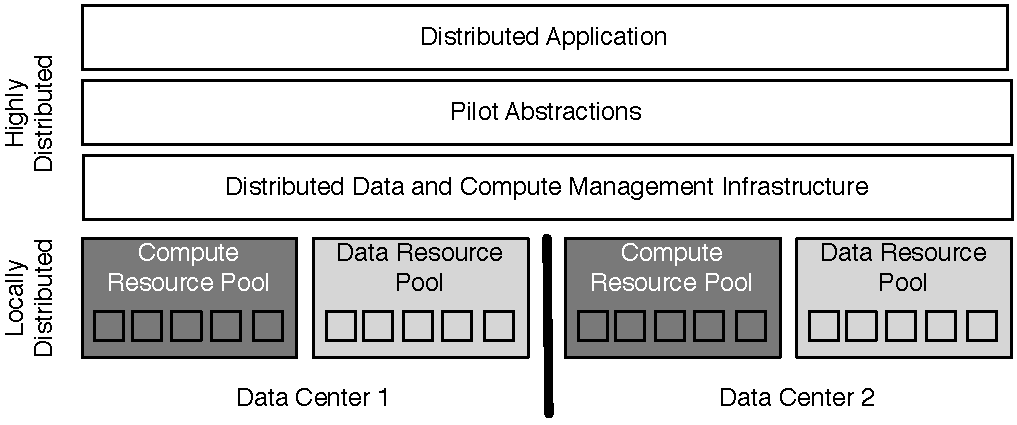
\includegraphics[width=0.45\textwidth]{figures/terminology.pdf}
	\caption{Levels of Distribution}
	\label{fig:figures_terminology}
\end{figure}

Figure~\ref{fig:figures_terminology} illustrates the possibly degree of 
distributions.


\section{Related Work}

Several different tools, e.\,g.
BitDew~\cite{Fedak:2008:BPE:1413370.1413416}, SRM~\cite{srm-ogf},
iRODS~\cite{Rajasekar:2010:IPI:1855046}, Condor
Matchmaking~\cite{Raman:1998:MDR:822083.823222} and
HDFS/Hadoop~\cite{hadoop}, address the general ideas associated with
affinity, most of the tools introduce the concept in semantically
inconsistent and implicit ways; consequently, affinities are not one
of the degrees-of-freedom exposed to or controllable at the
application-level (i.e.  by the developer/user). Furthermore, few
existing (distributed) programming models provide explicit support or
control for affinity~\cite{ideas}.



\subsection{Storage Infrastructure}

In distributed settings, storage is often a black box for the application with
unknown quality of services, i.\,e. the application usually does not know what
bandwidths and latencies it can expect. Furthermore, physical and logical
distribution implies higher penalties for inefficient data access as the data
traverses several hardware and software layers.


In general, different types of storage exist (see 
figure~\ref{fig:figures_storage-types}):

\begin{enumerate}
	\item \textbf{Local Storage:} describes local hard disk directly attached 
	to the compute resource.
	\item \textbf{Network Filesystem:} refers to different forms of 
	distributed (possible parallel) filesystems. The filesystem is commonly 
	exported via the Posix API and a virtual filesystem layer.
	\item \textbf{Distributed Storage:} refers to a highly distributed type of 
	storage systems that spawn across multiple data centers. Access to such 
	storage systems via a common -- often simplified -- namespace and API. For 
	example, cloud systems, such as the Azure Blob Storage, Amazon S3 and 
	Google Storage, provide only a namespace with a 1-level hierarchy. 
\end{enumerate}

While the coupling between compute and data in type 1 and 2 is very high, it 
is only small in the later case. In general, the buffer type 3 storage are 
more optimized to reliably storing large volumes of data and achieving high
read throughputs.

\alnote{Why do we exclude databases?}

\begin{figure}[t]
	\centering
		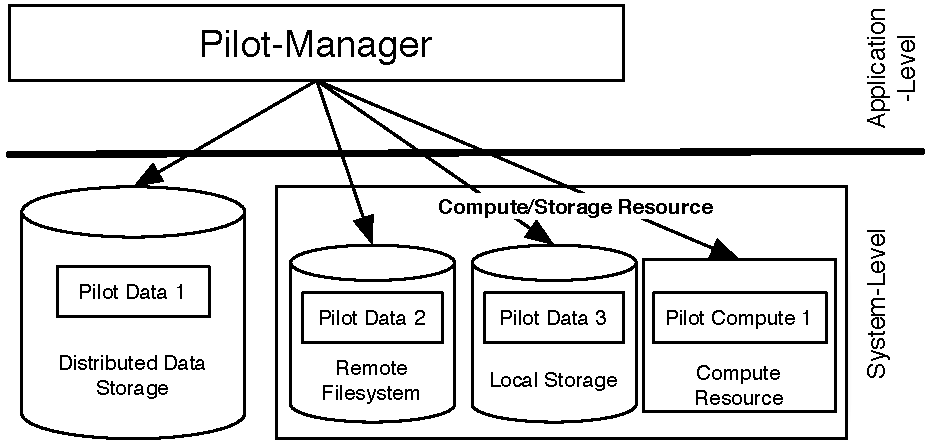
\includegraphics[width=0.45\textwidth]{figures/storage-types.pdf}
	\caption{Pilot-Compute and Pilot-Data on Different Types of Storage Resources}
	\label{fig:figures_storage-types}
\end{figure}



Table~\ref{tab:storage-systems} shows an overview of distributed storage 
systems. The focus of this analysis are file-based storage systems. Structured
storage types (e.g. relational databases) and key-/values stores are not 
considered.

\begin{table}[t]
\begin{tabular}{|p{1.3cm}|p{1cm}|p{1cm}|p{1cm}|p{1cm}|p{1cm}|}
	\hline
	\textbf{Storage Type} &\textbf{Azure} &\textbf{Amazon} &\textbf{Google} &\textbf{XSEDE}  &\textbf{OSG} \\
	\hline
	Local	&yes &yes &yes &yes &yes\\
	\hline
	Network Filesystem &Azure Drive &EBS &GCE Block Storage &Lustre, GPFS 
	&no\\
	\hline
	Distributed Storage &Azure Blob Storage &S3 &Google Storage &GFFS
	 &SRM\\
	\hline	
\end{tabular}
\caption{File-based storage types for different infrastructures (key/value and 
SQL-based storage types omitted) \label{tab:storage-systems}}
\end{table}


\subsection{Storage Backends}

Criteria/Requirements:
\begin{itemize}
	\item unstructured vs. semi-structured vs. structured data
	\item Volume of the data
	\item Access patterns
\end{itemize}

These data store types are suitable mainly for structured/semi-structured and 
medium size data:
\begin{itemize}
	\item In-memory, key-value Stores
	\item Document Stores like MongoDB, CouchDB 
	\item SQL-based databases
\end{itemize}

Scale-out data stores for BigData:
\begin{itemize}
	\item Swift
	\item Walrus
	\item Cassandra
	\item Hadoop: HDFS/HBase
\end{itemize}

TODO: How can this be used to implement affinities?


\subsection{Distributed Storage Systems}

iRods
SRM


While some distributed storage systems provide support for data/compute 
co-location (e.\,g.\ iRODS~\cite{Rajasekar:2010:IPI:1855046}), commonly 
applications require a direct access to files via a Posix-based API.

\subsection{Affinity}

How is affinity implemented in the above system

%%%%%%%%%%%%%%%%%%%%%%%%%%%%%%%%%%%%%%%%%%%%%%%%%%%%%%%%%%%%%%%%%%%%%%%%%%%%%%


\section{Pilot-Data}

We propose the use of \pilotdata as an application-level construct support
distributed data. In conjunction with \pilotjob, \pilotdata is able to support
different forms of data/compute affinities. Both abstractions are implemented
as reference implementation to the P* model -- a unifying, analytical
framework for \pilot abstractions -- introduced in~\cite{pstar11}. 
Similarly to \pilotjobs, \pilotdata allows the logical decoupling
of production and consumption of data. Among many things, \pilotdata 
facilitates the late binding of data and physical resources.  

\subsection{Affinities Overview}

An important consequence of data and computation as equal first-class
entities, is that either data (D) can be provisioned where computation
(C) is scheduled to take place (as is done traditionally), or C can be
provisioned where D resides. This equal movement of computational
units leads to a richer set of possible correlations between the
involved data elements and computational units; correlations can be
either spatial and/or temporal. These correlations arise either as a
consequence of constraints of localization (e.g., D is fixed, C must
move, or vice-versa), or as temporal ordering imposed on the different
data and computational units.


\subsection{\pilot-Abstractions and Affinities}


We use a simple model to describe resource affinities (see
figure~\ref{fig:figures_resource-topologies}). Data centers and machines are
represented as a tree. The further the distance between two resources, the
smaller the affinity.

\begin{figure}[t]
	\centering
		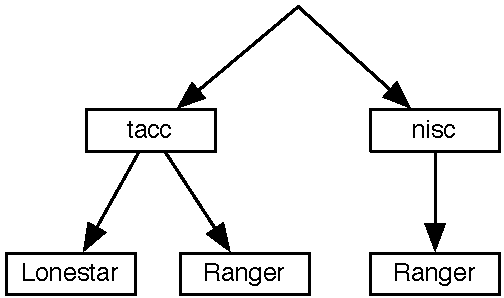
\includegraphics[width=0.3\textwidth]{figures/resource-topologies.pdf}
	\caption{\textbf{Modeling Resource Affinities:} Resources are placed in a 
	tree consisting of two levels. The smaller the distance between two 
	resources, the larger the affinity.}
	\label{fig:figures_resource-topologies}
\end{figure}

Each \pilot can specified the required affinity in it's description (see
listing~\ref{lst:pilot_compute_affinity}).

\begin{code}[
caption={Creation of a \textit{PilotCompute} on the specified  compute
resource endpoint.},
label={lst:pilot_compute_affinity}]
pilot_compute_description = 

{
    "service_url":"sge+ssh://gsissh.kraken.nics.xsede.org",
    "number_of_processes": 1,                             
    "working_directory": "/tmp/pilot-compute/",
    "affinity_datacenter_label": "nisc",              
    "affinity_machine_label": "kraken" 
}
\end{code}

The runtime system will map the requirements of the \pilot with an appropriate
resources (see figure~\ref{fig:figures_pilot-affinities}). Once a \pilot is
assigned to a resource, it inherits the affinity of that resource.

\begin{figure}[t]
	\centering
	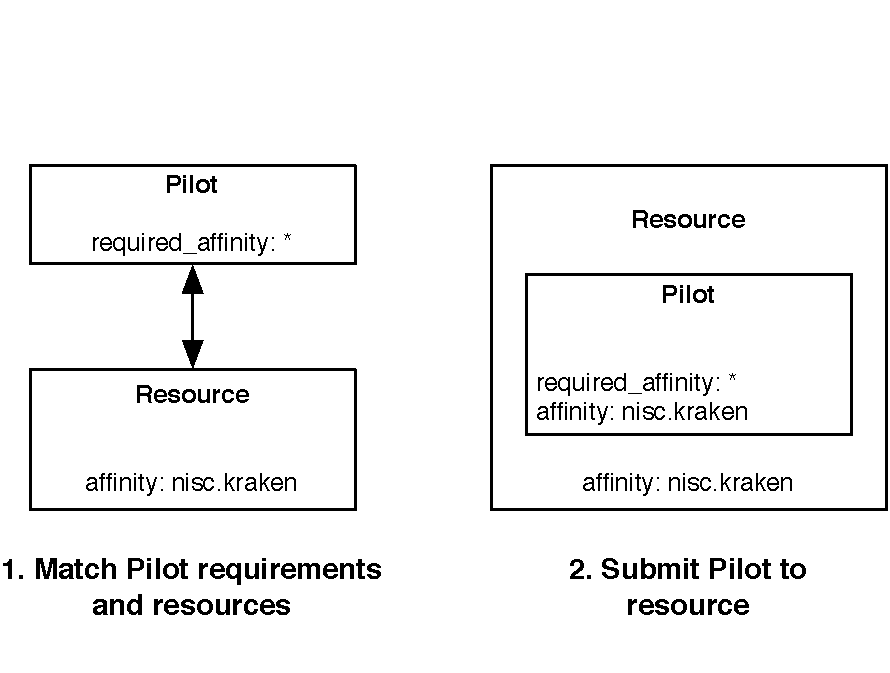
\includegraphics[width=0.45\textwidth]{figures/pilot-affinities.pdf}
	\caption{\pilot-Abstractions and Affinities}
	\label{fig:figures_pilot-affinities}
\end{figure}


In most cases it is necessary to co-locate \cus and \dus, i.\,e.\ either a \du
must be copied into a \pd that is placed on the same resource as the \pj or
vice versa. The other option is to stream the \du to the respective \cu.

TODO
explain how affinities can be used to model different storage types from section III

\subsection{Scheduling}

Comparison to YARN-based applications:
\begin{itemize}
	\item memory is primary scheduling objectives
	\item data-locality is not per definition taken care of application must 
	introspect HDFS for location of chunks and then request an appropriate 
	container
\end{itemize}


\subsection{BigData -- A PilotData Implementation}


The Pilot-Manager decides how and when to place data and
schedule its movement. Facilities provided include the creation of a
PD, the insertion/retrieval of \dataunits, and attachment to a storage
pool to hold its objects. Some implementation issues that need to be
understood and reasoned about include:

% The PD abstraction is designed to support the following capabilities:

%\begin{itemize}
\begin{compactitem}
\item \textbf{Distributed coupling and coordination:} Application
  components, e.\,g.\ the parts of a distributed workflow or a
  compute- and analysis job, need support for efficient distributed
  coordination.
\item \textbf{Description and management of data affinities and
    localities:} A \pd container represents a group of affine
  \dataunits; %Further affinities between several PD can be expressed;
  various meta-data, such as localities of all \dataunits and
  replicas, must be stored to facilitate scheduling and other types of
  decision making.
\item \textbf{Data-aware scheduling:} Utilizing the hints given to PD
  in form of affinity specifications, the data-aware scheduler should
  be able to optimize data localities, movements and
  streams. Depending on the current system state, computations will be
  moved to data or vice versa. Replicas of \dataunits can be
  automatically maintained by PD to facilitate e.\,g.\ a faster
  access.
\item \textbf{Data access patterns and data streaming:} Data contained
  within PD needs to be accessed online and streamed to different
  locations facilitating e.\,g.\ interactive analyses.  PD should
  support common data access patterns, e.\,g.\ replication,
  partitioning and scatter/gather.
\item \textbf{Discovery:} Application components should be able to
  query the system for \dataunits and their associated
  \pilots. Further, the system will provide support for shared \dus,
  which can be queried and discovered.
\end{compactitem}

The abstractions enables the
developer to specify data affinities, which will be utilized by the RTS to
map data onto a particular infrastructure topology and to support an
application-specific access pattern, e.\,g.\ as found in MapReduce
applications. The RTS places \dataunits according to the defined
objectives; for example, a resource could accept only data objects
$>5$~GB and above.  Ref.~\cite{ddia_ptrsa10} suggests that the
explicit support for affinities between and within the \pj and \pd
abstractions for distributed and dynamic data will yield better
performance and scalability compared to simplistic if not ad-hoc ways
of data-compute coupling while still maintaining a high level of
simplicity.


\begin{itemize}

\item Similar levels of heterogeneity in the data infrastructure

\begin{itemize}
\item File systems, storage, transport protocols, …
\end{itemize}

\item Support application level capabilities to specify dependencies
  at a logical level rather than specific file level

\begin{itemize}
\item First class support for Affinities (D-C, D-D)
\end{itemize}

\item Typically placement and scheduling of data is decoupled from the compute-tasks

\begin{itemize}
\item Integrated approach to compute and data ?
\end{itemize}

\item Dynamic decision for data

\begin{itemize}
\item Analogous  to late-binding of data
\item Fluctuating resources as a fundamental property of DCI
\end{itemize}

\item Abstraction for other factors and not application specific way
\begin{itemize}
\item Varying data sources, fluctuating data rates, etc
\end{itemize}

\end{itemize}

Reasoning about PilotData

\subsection{Implementation}
Substantiate with description of design decisions


\begin{table}[t]
	\centering
\begin{tabular}{|p{1.3cm}|p{1cm}|p{1cm}|p{1cm}|p{1cm}|p{1cm}|}
	\hline
	&\textbf{XSEDE} &\textbf{SRM} &\textbf{iRODS} &\textbf{Clouds} &\textbf{Hadoop}\\
	\hline
Pilot &Filesystem directory &SRM directory referenced by SURL & &Bucket&HDFS Directory\\
	\hline
DataUnit &&&&&HDFS Chunk\\
ComputeUnit &&&&&YARN App Container\\
	\hline
\end{tabular}
\caption{Mapping of Pilot Data to different infrastructures (clouds refer to Google Storage/Amazon S3/Microsoft Blob Storage)}
\end{table}

In general, SRM works on individual file basis \alnote{Can SRM work on directories or group of files?}.


\begin{table}[ht]
\begin{tabular}{|p{1cm}|p{1cm}|p{1cm}|p{1cm}|p{1cm}|p{1cm}|}
		\hline
		&\textbf{XSEDE} &\textbf{SRM} &\textbf{iRODS} &\textbf{Clouds} &\textbf{Hadoop}\\
		\hline
		Transfer &SCP, GridFTP &GridFTP &GridFTP &HTTP &HDFS, HTTP\\
		\hline
		Storage &VFS, GFFS &Storage Element & &S3, GS &\\
		\hline
\end{tabular}
\caption{File Transfer Protocols}
\end{table}


Push vs. Pull data

High-Level abstraction on to of logical/abstract file name 





\section{Pilot-API}
Pilot-API provides a unified interface for both \pilotcompute and \pilotdata 
capabilities.


\texttt{ComputeUnitContext}: Can be used by compute unit to query 



\section{Experiments}

How do we support affinity?

PD on heterogeneous backends

Distributed systems/data

Similar coordination graph as in the past

"Intelligent" data placements:

- ComputeDataService decides whether data, compute or both have to move

- 3 different cases:

i) move all data everywhere

ii) move data when task has been placed

iii) move data and then place task

Assumption:
How is initial data placed?
- distributed
- central in one place

Second application track:
- Data movement in the context of MD jobs

Which application?
- exclusively bfast?
- bwa? another good application?
- in some cases reference data is decomposable...

Look at the difference in $T_c$ for each application in the three
cases. We might introduce the idea of alpha. We dont' need to
quantify, but can qualitatively show how alpha determines the
importance (as measured by time to solution). 

My hunch is that $T_c$ will be more sensitive for data-intensive
application than other way around.

The idea is that for an application which is



\section{Conclusion and Future Work}

\section*{Acknowledgements}
%\up
\footnotesize \footnotesize{This work is funded by NSF CHE-1125332
  (Cyber-enabled Discovery and Innovation), HPCOPS NSF-OCI 0710874
  award, NSF-ExTENCI (OCI-1007115) and ``Collaborative Research:
  Standards-Based Cyberinfrastructure for Hydrometeorologic Modeling:
  US-European Research Partnership'' (OCI-1235085).  MS is sponsored
  by the program of BiG Grid, the Dutch e-Science Grid, which is
  financially supported by the Netherlands Organisation for Scientific
  Research, NWO. SJ acknowledges useful related discussions with Jon
  Weissman (Minnesota) and Dan Katz (Chicago). We thank J Kim (CCT)
  for assistance with BFAST.  This work has also been made possible
  thanks to computer resources provided by TeraGrid TRAC award
  TG-MCB090174 (Jha) and BiG Grid.  This document was developed with
  support from the US NSF under Grant No. 0910812 to Indiana
  University for ``FutureGrid: An Experimental, High-Performance Grid
  Test-bed''.}

  
\bibliographystyle{IEEEtran}
\bibliography{literatur,saga,saga-related,local}


\end{document}

